\documentclass[12pt]{article}

\usepackage{times}
\usepackage{graphicx}
\usepackage{amsmath}
\usepackage{url}

\setlength{\textwidth}{6.5in}
\setlength{\textheight}{8.9in}
\setlength{\oddsidemargin}{0.0in}
\setlength{\topmargin}{0.05in}
\setlength{\headheight}{-0.05in}
\setlength{\headsep}{0.0in}

\newcommand{\indep}{\perp\!\!\!\perp}

\begin{document}

\begin{center}
{\bf CS 6300} \hfill {\large\bf HW09: VPI and HMMs \hfill Due April 18, 2017}
\end{center}

\noindent
Please use the \LaTeX\ template to produce your writeups. See the
Homework Assignments page on the class website for details.  Hand in
at: \url{https://webhandin.eng.utah.edu/index.php}.

\section{Decision Networks and VPI}

\begin{center}
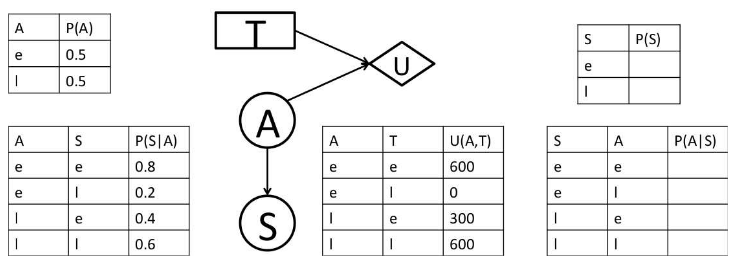
\includegraphics[width=6in]{prob1.png}
\end{center}

Your parents are visiting you for graduation.  You are in charge of
picking them up at the airport.  Their arrival time ($A$) might be
early ($e$) or late ($l$).  You decide on a time ($T$) to go to the
airport, also either early ($e$) or late ($l$).  Your sister ($S$) is
a noisy source of information about their arrival time. The
probability values and utilities are shown in the tables above.

Compute $P(S), P(A|S)$ and compute the quantities below. 

\begin{enumerate}

\item $EU(T=e)$

\item $EU(T=l)$

\item $MEU( \{ \} )$

\item Optimal action with no observations

\end{enumerate}

\noindent
Now we consider the case where you decide to ask your sister for input.

\begin{enumerate}

\item $EU(T=e | S = e)$

\item $EU(T=l | S = e)$

\item $MEU( \{ S=e \} )$

\item Optimal action with observation $\{S = e\}$

\item $EU(T = e | S = l)$

\item $EU(T = l | S = l)$

\item $MEU( \{ S=l \} )$

\item Optimal action with observation $S = l$

\item $VPI(S)$

\end{enumerate}

\section{Wherefore art thou Romeo?}

Romeo and Juliet are two lovesick robots; they function best when each
knows where the other is.  Romeo has become lost, and is trying to
figure out where he is so he can tell Juliet.  Romeo is on the grid
below, which also lists transition probabilities and properties of the
sensors.  At each step, Romeo senses, and then transitions to an
adjacent room to get to the next time step.  Romeo observed the
following evidence while wandering in grief over his inability to tell
Juliet where he is: 2 walls, 2 walls, 3 walls.

\begin{description}

\item[Forward Algorithm] Compute the most likely location, given the evidence.

\item[Viterbi Algorithm] Compute the most likely sequence of steps he
  took in the maze for the above evidence.

\end{description}

\clearpage

\begin{center}
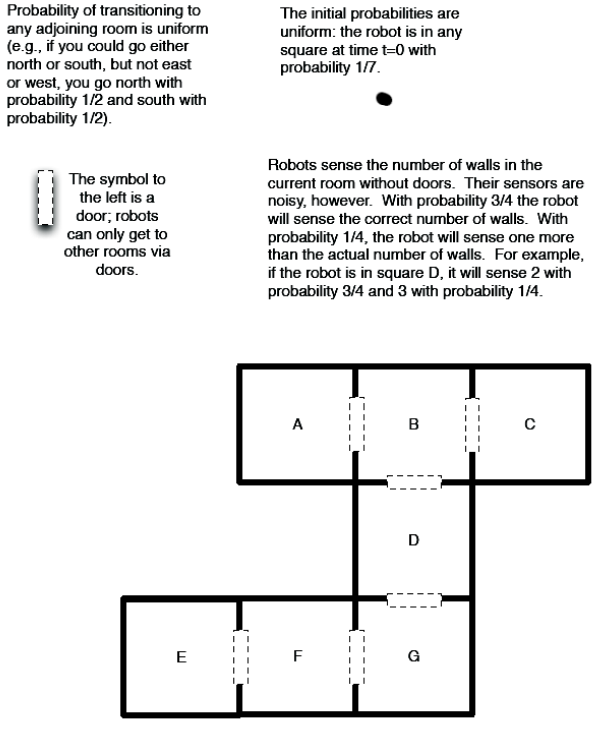
\includegraphics[height=7in]{prob2.png}
\end{center}

\end{document}


